% Connection problem illustration – identical topology to problem-illustration.tex.
% Terminals U = {v1, v5, v8} drawn with double circle.
% Steiner vertices used in solution (v4, v10) drawn with dashed border.
% Steiner tree: v1 -[blue]- v10 -[blue]- v4 -[orange]- v5
%                                v10 -[green]- v8
\begin{minipage}[t]{0.49\linewidth}
\centering
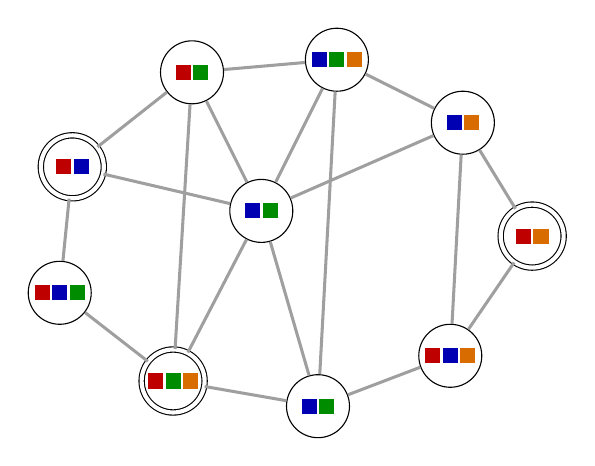
\begin{tikzpicture}[scale=0.80]
    \colorlet{iface1}{red!75!black}
    \colorlet{iface2}{blue!70!black}
    \colorlet{iface3}{green!55!black}
    \colorlet{iface4}{orange!85!black}

    % non-terminal, non-Steiner vertices
    \node[circle, draw, minimum size=8mm, inner sep=0pt] (v2)  at (1.9, 2.7) {};
    \node[circle, draw, minimum size=8mm, inner sep=0pt] (v3)  at (4.2, 2.9) {};
    \node[circle, draw, minimum size=8mm, inner sep=0pt] (v6)  at (6.0,-1.8) {};
    \node[circle, draw, minimum size=8mm, inner sep=0pt] (v7)  at (3.9,-2.6) {};
    \node[circle, draw, minimum size=8mm, inner sep=0pt] (v9)  at (-0.2,-0.8) {};
    % terminal vertices (double circle)
    \node[circle, draw, double, double distance=1.5pt,
          minimum size=8mm, inner sep=0pt] (v1) at (0.0, 1.2) {};
    \node[circle, draw, double, double distance=1.5pt,
          minimum size=8mm, inner sep=0pt] (v5) at (7.3, 0.1) {};
    \node[circle, draw, double, double distance=1.5pt,
          minimum size=8mm, inner sep=0pt] (v8) at (1.6,-2.2) {};
    % Steiner vertices in the solution
    \node[circle, draw, minimum size=8mm, inner sep=0pt] (v4)  at (6.2, 1.9) {};
    \node[circle, draw, minimum size=8mm, inner sep=0pt] (v10) at (3.0, 0.5) {};

    % all edges – thin gray
    \draw[gray!75, line width=1.1pt] (v1) -- (v2) -- (v3) -- (v4) -- (v5) -- (v6) -- (v7) -- (v8) -- (v9) -- (v1);
    \draw[gray!75, line width=1.1pt] (v1) -- (v10);
    \draw[gray!75, line width=1.1pt] (v2) -- (v10);
    \draw[gray!75, line width=1.1pt] (v3) -- (v10);
    \draw[gray!75, line width=1.1pt] (v4) -- (v10);
    \draw[gray!75, line width=1.1pt] (v7) -- (v10);
    \draw[gray!75, line width=1.1pt] (v8) -- (v10);
    \draw[gray!75, line width=1.1pt] (v2) -- (v8);
    \draw[gray!75, line width=1.1pt] (v3) -- (v7);
    \draw[gray!75, line width=1.1pt] (v4) -- (v6);

    % available interface rectangles (identical to problem-illustration.tex)
    \begin{scope}[shift={(v1.center)}]
        \fill[iface1] (-0.26,-0.12) rectangle (-0.02,0.12);
        \fill[iface2] (0.02,-0.12) rectangle (0.26,0.12);
    \end{scope}
    \begin{scope}[shift={(v2.center)}]
        \fill[iface1] (-0.26,-0.12) rectangle (-0.02,0.12);
        \fill[iface3] (0.02,-0.12) rectangle (0.26,0.12);
    \end{scope}
    \begin{scope}[shift={(v3.center)}]
        \fill[iface2] (-0.40,-0.12) rectangle (-0.16,0.12);
        \fill[iface3] (-0.12,-0.12) rectangle (0.12,0.12);
        \fill[iface4] (0.16,-0.12) rectangle (0.40,0.12);
    \end{scope}
    \begin{scope}[shift={(v4.center)}]
        \fill[iface2] (-0.26,-0.12) rectangle (-0.02,0.12);
        \fill[iface4] (0.02,-0.12) rectangle (0.26,0.12);
    \end{scope}
    \begin{scope}[shift={(v5.center)}]
        \fill[iface1] (-0.26,-0.12) rectangle (-0.02,0.12);
        \fill[iface4] (0.02,-0.12) rectangle (0.26,0.12);
    \end{scope}
    \begin{scope}[shift={(v6.center)}]
        \fill[iface1] (-0.40,-0.12) rectangle (-0.16,0.12);
        \fill[iface2] (-0.12,-0.12) rectangle (0.12,0.12);
        \fill[iface4] (0.16,-0.12) rectangle (0.40,0.12);
    \end{scope}
    \begin{scope}[shift={(v7.center)}]
        \fill[iface2] (-0.26,-0.12) rectangle (-0.02,0.12);
        \fill[iface3] (0.02,-0.12) rectangle (0.26,0.12);
    \end{scope}
    \begin{scope}[shift={(v8.center)}]
        \fill[iface1] (-0.40,-0.12) rectangle (-0.16,0.12);
        \fill[iface3] (-0.12,-0.12) rectangle (0.12,0.12);
        \fill[iface4] (0.16,-0.12) rectangle (0.40,0.12);
    \end{scope}
    \begin{scope}[shift={(v9.center)}]
        \fill[iface1] (-0.40,-0.12) rectangle (-0.16,0.12);
        \fill[iface2] (-0.12,-0.12) rectangle (0.12,0.12);
        \fill[iface3] (0.16,-0.12) rectangle (0.40,0.12);
    \end{scope}
    \begin{scope}[shift={(v10.center)}]
        \fill[iface2] (-0.26,-0.12) rectangle (-0.02,0.12);
        \fill[iface3] (0.02,-0.12) rectangle (0.26,0.12);
    \end{scope}
\end{tikzpicture}

\vspace{1mm}
{\scriptsize Available labels (double contour = terminal)}
\end{minipage}
\hfill
\begin{minipage}[t]{0.49\linewidth}
\centering
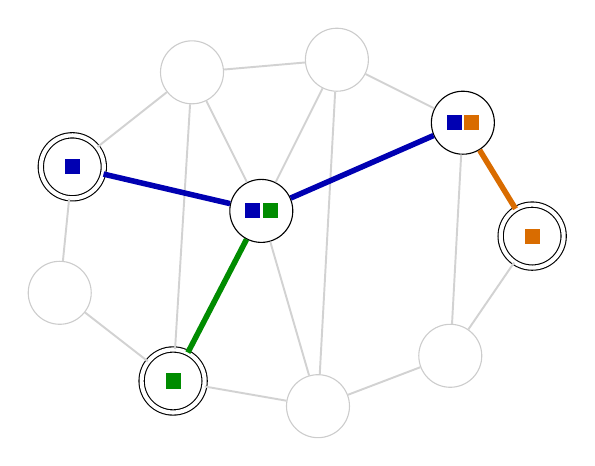
\begin{tikzpicture}[scale=0.80]
    \colorlet{iface1}{red!75!black}
    \colorlet{iface2}{blue!70!black}
    \colorlet{iface3}{green!55!black}
    \colorlet{iface4}{orange!85!black}

    % non-terminal, non-Steiner vertices (faded)
    \node[circle, draw=gray!40, minimum size=8mm, inner sep=0pt] (v2)  at (1.9, 2.7) {};
    \node[circle, draw=gray!40, minimum size=8mm, inner sep=0pt] (v3)  at (4.2, 2.9) {};
    \node[circle, draw=gray!40, minimum size=8mm, inner sep=0pt] (v6)  at (6.0,-1.8) {};
    \node[circle, draw=gray!40, minimum size=8mm, inner sep=0pt] (v7)  at (3.9,-2.6) {};
    \node[circle, draw=gray!40, minimum size=8mm, inner sep=0pt] (v9)  at (-0.2,-0.8) {};
    % terminal vertices (double circle)
    \node[circle, draw, double, double distance=1.5pt,
          minimum size=8mm, inner sep=0pt] (v1) at (0.0, 1.2) {};
    \node[circle, draw, double, double distance=1.5pt,
          minimum size=8mm, inner sep=0pt] (v5) at (7.3, 0.1) {};
    \node[circle, draw, double, double distance=1.5pt,
          minimum size=8mm, inner sep=0pt] (v8) at (1.6,-2.2) {};
    % Steiner vertices used in solution
    \node[circle, draw, minimum size=8mm, inner sep=0pt] (v4)  at (6.2, 1.9) {};
    \node[circle, draw, minimum size=8mm, inner sep=0pt] (v10) at (3.0, 0.5) {};

    % non-tree edges (thin, faded)
    \draw[gray!35, line width=0.7pt] (v1) -- (v2) -- (v3) -- (v4) -- (v5) -- (v6) -- (v7) -- (v8) -- (v9) -- (v1);
    \draw[gray!35, line width=0.7pt] (v2) -- (v10);
    \draw[gray!35, line width=0.7pt] (v3) -- (v10);
    \draw[gray!35, line width=0.7pt] (v7) -- (v10);
    \draw[gray!35, line width=0.7pt] (v2) -- (v8);
    \draw[gray!35, line width=0.7pt] (v3) -- (v7);
    \draw[gray!35, line width=0.7pt] (v4) -- (v6);

    % Steiner tree edges (thick, coloured by activated interface)
    \draw[iface2, line width=2.0pt] (v1)  -- (v10); % iface2 (blue)
    \draw[iface2, line width=2.0pt] (v10) -- (v4);  % iface2 (blue)
    \draw[iface4, line width=2.0pt] (v4)  -- (v5);  % iface4 (orange)
    \draw[iface3, line width=2.0pt] (v10) -- (v8);  % iface3 (green)

    % assigned interfaces (solution only)
    \begin{scope}[shift={(v1.center)}]
        \fill[iface2] (-0.12,-0.12) rectangle (0.12,0.12);
    \end{scope}
    \begin{scope}[shift={(v4.center)}]
        \fill[iface2] (-0.26,-0.12) rectangle (-0.02,0.12);
        \fill[iface4] (0.02,-0.12) rectangle (0.26,0.12);
    \end{scope}
    \begin{scope}[shift={(v5.center)}]
        \fill[iface4] (-0.12,-0.12) rectangle (0.12,0.12);
    \end{scope}
    \begin{scope}[shift={(v8.center)}]
        \fill[iface3] (-0.12,-0.12) rectangle (0.12,0.12);
    \end{scope}
    \begin{scope}[shift={(v10.center)}]
        \fill[iface2] (-0.26,-0.12) rectangle (-0.02,0.12);
        \fill[iface3] (0.02,-0.12) rectangle (0.26,0.12);
    \end{scope}
\end{tikzpicture}

\vspace{1mm}
{\scriptsize Example connecting assignment}
\end{minipage}
